\chapter{State of the Art}
\section{Censorship Mechanisms \& Circumvention Techniques}



\section{Ireland}

\subsection{Censorship in the Past}

According to a report from the United States Department of State in 2011, it was found that there were no government restrictions on access to the internet or that the government actively monitored email or internet chatrooms \cite{stateTechnicalDifficulties}.

The Irish government engages in censoring or blocking the distribution of pirated copryrighted material. In 2009, the Irish Telecom Company, EIRCOM, blocked its customers from accessing the website \textit{The Pirate Bay}. The Pirate Bay is a Swedish website which provides links to copyrighted material. The website was hit with a lawsuit from major record labels and many ISPs around the world agreed to block access to the website as part of the settlement. However, not all Irish ISPs complied. The cable TV operator UPC announced that it would not comply \cite{irishtimesEircomBlock}. 

In alignment with international agreements, the Irish Government blocks access to websites that contain illegal content, such as Child Sexual Abuse Material (CSAM). The government has setup a hotline that allows citizens to anonymously report websites that they suspect contain illegal content, called hotline.ie \cite{hotlineAboutx2013}.

In contrast to other EU countries, Ireland does not have a broad government-mandated filtering system. They instead have the power through the Irish courts to mandate Irish ISPs to block certain websites. In addition, Irish ISPs may voluntarily enforce content filtering and website blocking in alignment with Irish content law.

Up until 2014, Ireland and other EU countries followed data retention laws, which required ISPs to store metadata for law enforcement purposes. In 2014, the European Court of Justice struck down the directive, which led to a change in this law in Ireland \cite{DataRetentionInvalid2014}. After this change, Ireland enacted the \textit{Communications (Retention of Data)(Amendment) Act 2022} \cite{irishlegalDataRetention}. This legislation allows for the general and indiscriminate retention of communications traffic and location data on the grounds of national security, where approved by a judge.

\subsection{Current Censorship}

As a whole, Ireland's censorship efforts are limited and specific. The government and ISPs target mainly illegal and pirated content. Some specific websites that have been blocked include 1337x, Eztv, BMovies, GoMovies, Putlocker, Rarbg, WatchFree, and Yts \cite{siliconrepublicMovieIndustry}. However, piracy websites are still widely accessible in Ireland.

It seems that Ireland has also rolled back blocks on some websites, such as Russian News outlets. Previously, the domain russia.tv, was blocked in Ireland. But as of 2025, it is able to be partially accessed. Based on data from the OONI project, there is evidence of TCP/IP blocking of this domain in Ireland. Based on the findings from OONI, this domain is able to be accessed when EIRCOM's root DNS server (AS5466, IP: 86.47.80.38) is used, but is blocked when accessed through Cloudflare's DNS server (AS14593, IP: 172.69.193.80).

\centerline{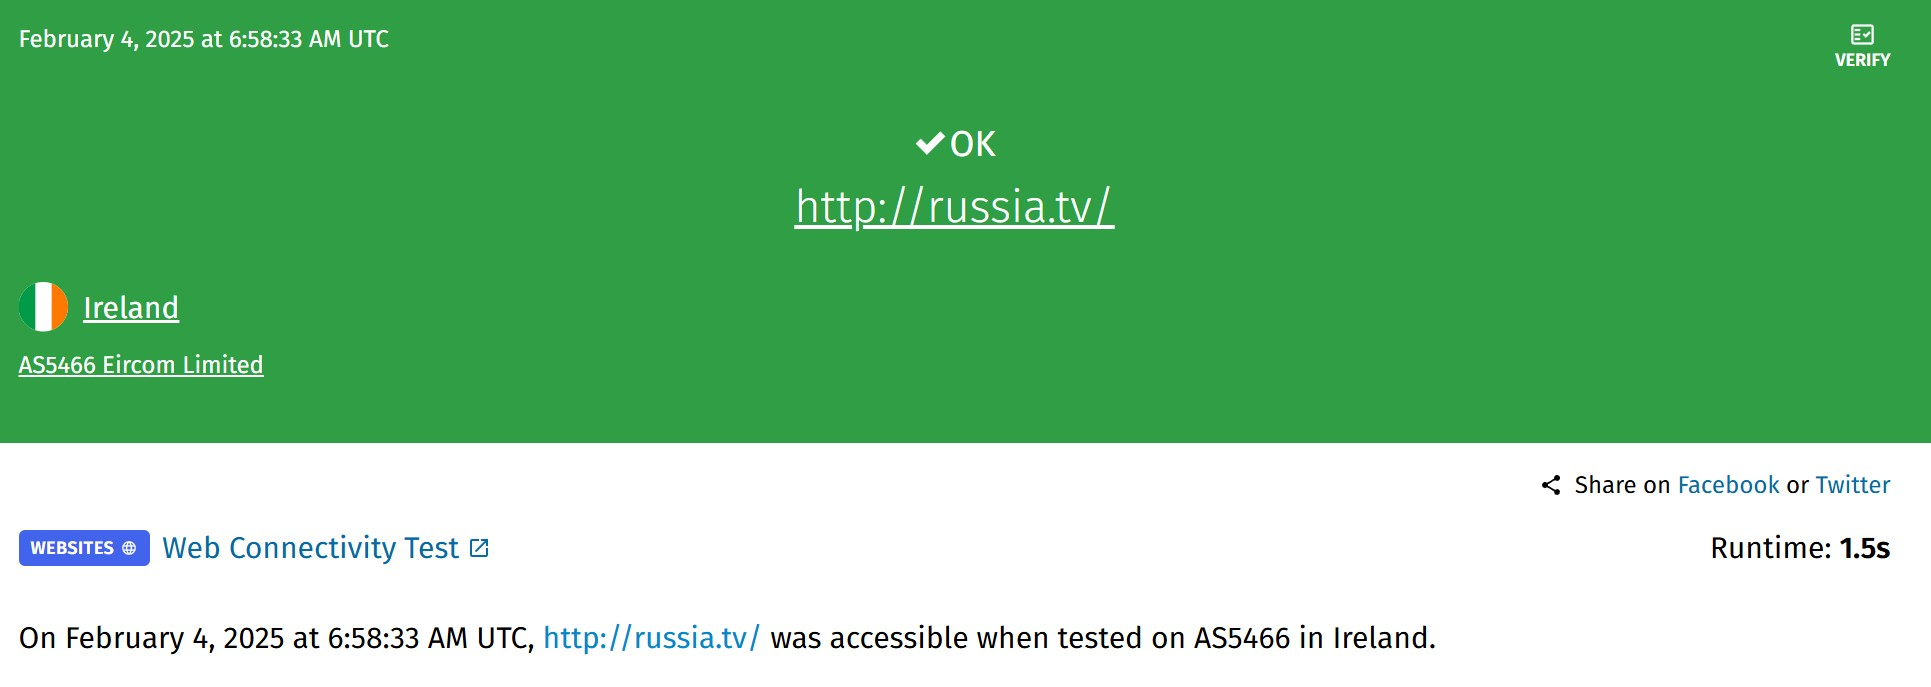
\includegraphics[width=480pt]{Griff/Latex/TCD SCSS CAPSTONE/Literature Review/Eircom Access russiatb.jpg}}

\centerline{\textit{Figure 1.1, EIRCOM DNS test for Russia.tv on OONI probe}}

\centerline{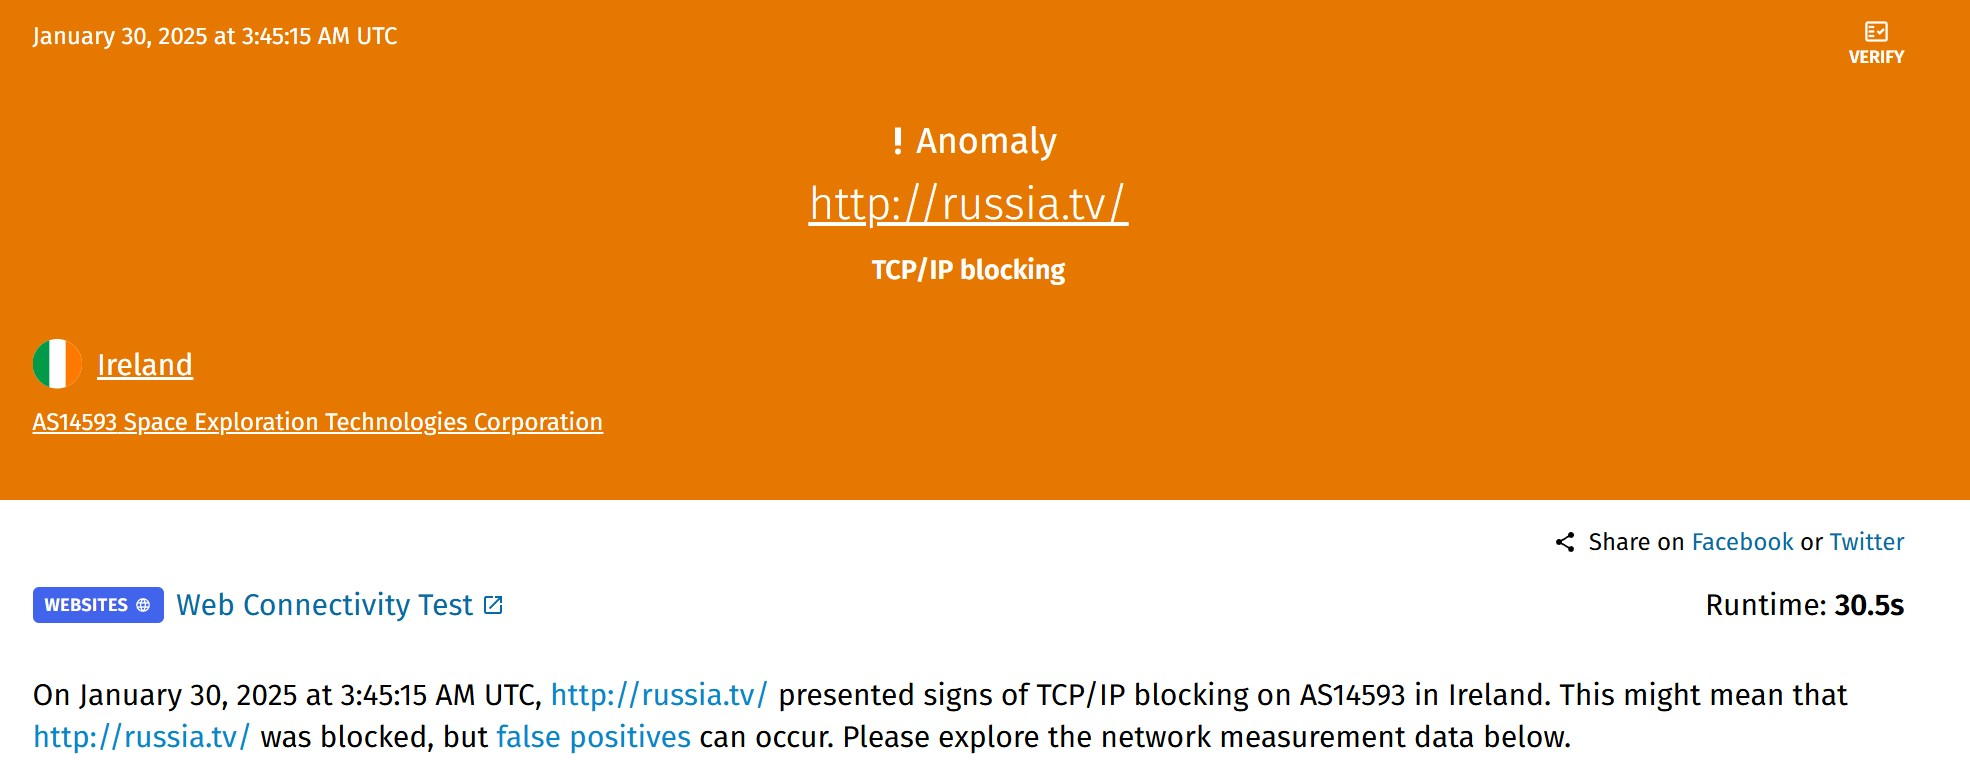
\includegraphics[width=480pt]{Griff/Latex/TCD SCSS CAPSTONE/Literature Review/CloudFlare Block Russiatv.jpg}}

\centerline{\textit{Figure 1.2, CloudFlare DNS test for Russia.tv on OONI probe}}

\centerline{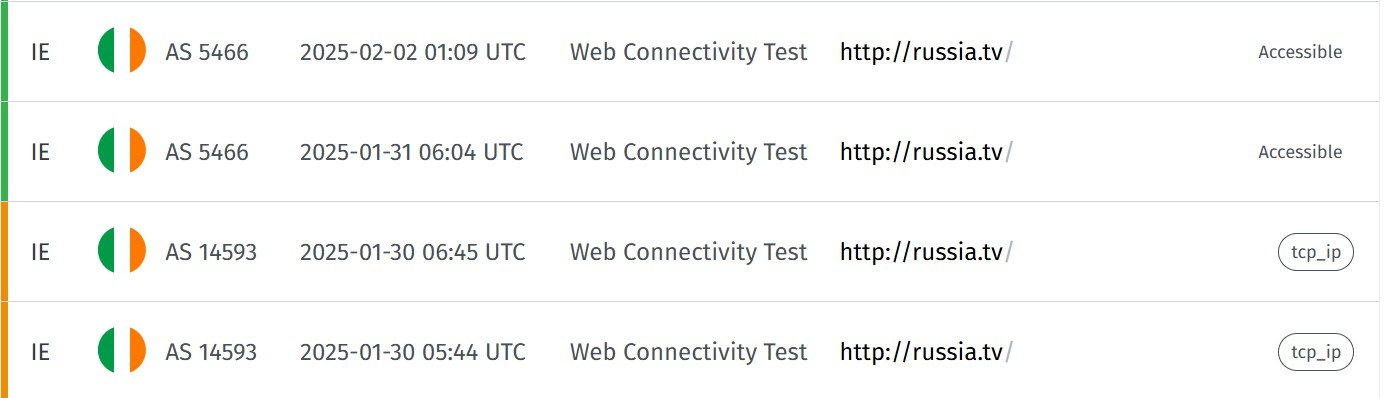
\includegraphics[width=480pt]{Griff/Latex/TCD SCSS CAPSTONE/Literature Review/RussiaTV search OONI.jpg}}

\centerline{\textit{Figure 1.3, Russia.tv domain search on OONI}}

\section{Iraq}

\section{Tools}

\subsection{The Tor Browser}

\subsection{VPNs}
